
\documentclass[11pt]{article}
\usepackage[11pt,inchmargins]{sigmin}
\usepackage[T1]{fontenc}
\usepackage{tgtermes}
\usepackage{atbegshi}
%\usepackage{showframe}

\usepackage{graphics}
\usepackage{epsfig}
\usepackage{xspace}
\usepackage[nolineno,noindent,norules]{lgrind}
\usepackage{subfig,graphics,graphicx,color}
\DeclareGraphicsExtensions{.eps}


% \def\v#1{{\texttt{\fontfamily{cmtt}\fontsize{\f@size}{\f@size}\selectfont #1}}}
\let\vv\texttt

%% Title stuff.
%\newcommand{\mytitle}[0]{\textbf {Stable Multithreading: \\
%A New Paradigm for Reliable and Secure Threads}}
%\newcommand{\mykeywords}[0]{Deterministic Multithreading, Stable 
%Multithreading, Reliability, Security, Software Model Checking,
%State Space Reduction, State Machine Replication}




%% Terminology of our own internal techniques.
\newcommand{\kakute}[0]{\textsc{Kakute}\xspace}
\newcommand{\confluence}[0]{\textsc{Confluence}\xspace}
\newcommand{\pig}[0]{\textsc{Pig}\xspace}
\newcommand{\hadoop}[0]{\textsc{Hadoop}\xspace}
\newcommand{\maat}[0]{\textsc{Maat}\xspace}
\newcommand{\chref}[1]{\S\ref{#1}}
\newcommand{\lazyp}[0]{Reference Propagation\xspace}
\newcommand{\tagcache}[0]{Tag Sharing\xspace}
\newcommand{\func}[1]{\textsc{#1}}


% Objective 1
\newcommand{\appsn}[0]{4\space}
\newcommand{\appeval}[0]{seven\xspace}
\newcommand{\overheadcomp}[0]{50\%\xspace}
\newcommand{\overheadmem}[0]{1x\xspace}
\newcommand{\dagfull}[0]{Directed acyclic graph\space}
\newcommand{\timelow}[0]{60\%\space}
\newcommand{\timehigh}[0]{4.5X\space}
\newcommand{\timeavg}[0]{32.3\%\space}


%% Systems and techniques names.
% \newcommand{\xxx}[0]{\textsc{Gaia}\xspace}
\newcommand{\paxos}[0]{\textsc{Paxos}\xspace}
\newcommand{\spaxos}[0]{S-Paxos\xspace}
\newcommand{\zookeeper}{ZooKeeper\xspace}
\newcommand{\libpaxos}{libPaxos\xspace}
\newcommand{\dare}{DARE\xspace}
\newcommand{\crane}{\textsc{Crane}\xspace}
\newcommand{\falcon}{\textsc{Apus}\xspace}
\newcommand{\tripod}{\textsc{Tripod}\xspace}
\newcommand{\mesos}{\textsc{Mesos}\xspace}

\newcommand{\dmt}[0]{DMT\xspace}
\newcommand{\smt}[0]{StableMT\xspace}
\newcommand{\smr}[0]{SMR\xspace}
\newcommand{\racepro}[0]{\textsc{RacePro}\xspace}
\newcommand{\tern}[0]{\textsc{Tern}\xspace}
\newcommand{\peregrine}[0]{\textsc{Peregrine}\xspace}
\newcommand{\parrot}[0]{\textsc{Parrot}\xspace}
\newcommand{\grace}[0]{Grace\xspace}
\newcommand{\coredet}[0]{\textsc{CoreDet}\xspace}
\newcommand{\kendo}[0]{Kendo\xspace}
\newcommand{\dthreads}[0]{\textsc{DThreads}\xspace}
\newcommand{\determinator}[0]{Determinator\xspace}
\newcommand{\dbug}[0]{\textsc{dbug}\xspace}
\newcommand{\ecosys}[0]{\parrot-\dbug}
\newcommand{\ldpreload}[0]{LD\_PRELOAD\xspace}

\newcommand{\mutexlock}[0]{\texttt{pthread\_mutex\_lock}\xspace}
\newcommand{\send}[0]{\texttt{send}\xspace}
\newcommand{\accept}[0]{\texttt{accept}\xspace}
\newcommand{\connect}[0]{\texttt{connect}\xspace}
\newcommand{\recv}[0]{\texttt{recv}\xspace}
\newcommand{\sockread}[0]{\texttt{read}\xspace}
\newcommand{\close}[0]{\texttt{close}\xspace}
\newcommand{\select}[0]{\texttt{select}\xspace}
\newcommand{\poll}[0]{\texttt{poll}\xspace}
\newcommand{\epoll}[0]{\texttt{epoll}\xspace}
\newcommand{\randfunc}[0]{\texttt{rand}\xspace}
\newcommand{\srandfunc}[0]{\texttt{srand}\xspace}
\newcommand{\gettimeofday}[0]{\texttt{gettimeofday}\xspace}
\newcommand{\us}[0]{\(\mu\text{s}\)\xspace}
%\newcommand{\N}[0]{$N$\xspace}
%\newcommand{\M}[0]{$M$\xspace}
%\newcommand{\C}[0]{$C$\xspace}
%\newcommand{\timev}[0]{\texttt{T_{v}}\xspace}

%% Application names.
\newcommand{\azure}{Microsoft Azure\xspace}
\newcommand{\libsafe}{Libsafe\xspace}
\newcommand{\apache}{Apache\xspace}
\newcommand{\clamav}{ClamAV\xspace}
\newcommand{\ab}{ApacheBench\xspace}
\newcommand{\mysql}{MySQL\xspace}
\newcommand{\sysbench}{SysBench\xspace}
\newcommand{\mplayer}[0]{{MPlayer}\xspace}
\newcommand{\mencoder}[0]{\v{mencoder}\xspace}
\newcommand{\pbzip}[0]{\v{PBZip2}\xspace}
\newcommand{\aget}[0]{\v{aget}\xspace}
\newcommand{\mongoose}[0]{\v{Mongoose}\xspace}
\newcommand{\pfscan}[0]{\v{pfscan}\xspace}
\newcommand{\fft}[0]{\v{fft}\xspace}
\newcommand{\luc}[0]{\v{lu\_cb}\xspace}
\newcommand{\lun}[0]{\v{lu\_ncb}\xspace}
\newcommand{\barnes}[0]{\v{barnes}\xspace}
\newcommand{\radix}[0]{\v{radix}\xspace}
\newcommand{\radiosity}[0]{\v{radiosity}\xspace}
\newcommand{\waters}[0]{\v{water-spatial}\xspace}
\newcommand{\watern}[0]{\v{water-nsquared}\xspace}
\newcommand{\oceanncp}[0]{\v{ocean}\xspace}
\newcommand{\oceancp}[0]{\v{ocean}\xspace}
\newcommand{\ocean}[0]{\v{ocean}\xspace}
\newcommand{\fmm}[0]{\v{fmm}\xspace}
\newcommand{\volrend}[0]{\v{volrend}\xspace}
\newcommand{\cholesky}[0]{\v{cholesky}\xspace}
\newcommand{\streamcluster}[0]{\v{streamcluster}\xspace}
\newcommand{\blackscholes}[0]{\v{blackscholes}\xspace}
\newcommand{\swaptions}[0]{\v{swaptions}\xspace}
\newcommand{\bodytrack}[0]{\v{bodytrack}\xspace}
\newcommand{\bodytrackopenmp}[0]{\v{bodytrack-openmp}\xspace}
\newcommand{\ferret}[0]{\v{ferret}\xspace}
\newcommand{\dedup}[0]{\v{dedup}\xspace}
\newcommand{\raytrace}[0]{\v{raytrace}\xspace}
\newcommand{\canneal}[0]{\v{canneal}\xspace}
\newcommand{\racey}[0]{\v{racey}\xspace}
\newcommand{\freqmine}[0]{\v{freqmine}\xspace}
\newcommand{\vips}[0]{\v{vips}\xspace}
\newcommand{\xtwosixfour}[0]{\v{x264}\xspace}
\newcommand{\fluidanimate}[0]{\v{fluidanimate}\xspace}
\newcommand{\facesim}[0]{\v{facesim}\xspace}
\newcommand{\rtviewraytrace}[0]{\v{rtview\_raytrace}\xspace}
\newcommand{\wordcount}[0]{\v{word\_count}\xspace}
\newcommand{\klee}[0]{\textsc{klee}\xspace}
\newcommand{\woodpecker}[0]{\textsc{woodpecker}\xspace}
\newcommand{\splashx}[0]{\mbox{SPLASH-2x}\xspace}
\newcommand{\splash}[0]{\mbox{SPLASH-2}\xspace}
\newcommand{\parsec}[0]{\mbox{PARSEC}\xspace}
\newcommand{\phoenix}[0]{\mbox{Phoenix}\xspace}
\newcommand{\pthread}[0]{\mbox{Pthreads}\xspace}

%% Application names (continue).
\newcommand{\kmeans}[0]{\v{kmeans}\xspace}
\newcommand{\kmeanspthread}[0]{\v{kmeans-pthread}\xspace}
\newcommand{\linearregre}[0]{\v{linear-regression}\xspace}
\newcommand{\linearregrepthread}[0]{\v{linear-regression-pthread}\xspace}
\newcommand{\matrixmult}[0]{\v{matrix-multiply}\xspace}
\newcommand{\matrixmultpthread}[0]{\v{matrix-multiply-pthread}\xspace}
\newcommand{\wordcnt}[0]{\v{word-count}\xspace}
\newcommand{\wordcntpthread}[0]{\v{word-count-pthread}\xspace}
\newcommand{\stringmatch}[0]{\v{string-match}\xspace}
\newcommand{\stringmatchpthread}[0]{\v{string-match-pthread}\xspace}
\newcommand{\histogram}[0]{\v{histogram}\xspace}
\newcommand{\histogrampthread}[0]{\v{histogram-pthread}\xspace}
\newcommand{\pca}[0]{\v{pca}\xspace}
\newcommand{\pcapthread}[0]{\v{pca-pthread}\xspace}

%% Application names (continue).
\newcommand{\partition}[0]{\mbox{\v{partition}}\xspace}
\newcommand{\nthelement}[0]{\mbox{\v{nth\_element}}\xspace}
\newcommand{\partialsort}[0]{\mbox{\v{partial\_sort}}\xspace}
\newcommand{\ua}[0]{\v{ua}\xspace}
\newcommand{\is}[0]{\v{is}\xspace}
\newcommand{\npb}[0]{\mbox{NPB}\xspace}
\newcommand{\imagick}[0]{\mbox{ImageMagick}\xspace}
\newcommand{\openldap}[0]{{OpenLDAP}\xspace}
\newcommand{\redis}[0]{{Redis}\xspace}
\newcommand{\memcached}[0]{{Memcached}\xspace}
\newcommand{\bdb}[0]{{Berkeley DB}\xspace}
\newcommand{\openmp}[0]{{OpenMP}\xspace}
\newcommand{\libgomp}[0]{\v{libgomp}\xspace}
\newcommand{\vtune}[0]{\v{VTune}\xspace}

%% concurrency attack study stats.
\newcommand{\noldattacks}[0]{46\xspace}
\newcommand{\nattacks}[0]{23\xspace}

%% imagick programs
\newcommand{\convertshear}[0]{\v{convert\_shear}\xspace}
\newcommand{\montage}[0]{\v{montage}\xspace}

\newcommand{\nprog}[0]{108\xspace}
\newcommand{\nrealprog}[0]{55\xspace}
\newcommand{\nstl}[0]{33\xspace}
\newcommand{\nimagick}[0]{14\xspace}
\newcommand{\nparsec}[0]{15\xspace}
\newcommand{\nphoenix}[0]{14\xspace}
\newcommand{\nsplash}[0]{14\xspace}
\newcommand{\nnpb}[0]{10\xspace}
\newcommand{\nbenchmarks}[0]{53\xspace}
\newcommand{\ndatapartition}[0]{86\xspace}
\newcommand{\nprogadhocsync}[0]{5\xspace}
\newcommand{\nprogtimeout}[0]{5\xspace}

\newcommand{\nprognohints}[0]{18\xspace}
\newcommand{\nprogneedhints}[0]{90\xspace}
\newcommand{\nprognondethints}[0]{9\xspace}
\newcommand{\nprognondetandnetwork}[0]{11\xspace} % the UA program is excluded.
\newcommand{\nprognonondethints}[0]{99\xspace}
\newcommand{\nproglineuphints}[0]{81\xspace}
\newcommand{\nproggenericlineuphints}[0]{43\xspace}
\newcommand{\nprogspecificlineuphints}[0]{38\xspace}
\newcommand{\nlineofhints}[0]{109\xspace}
\newcommand{\nlineofcomputehints}[0]{87\xspace}
\newcommand{\nlineofnondethints}[0]{22\xspace}
\newcommand{\hintsperprog}[0]{1.2\xspace}
\newcommand{\nlineupfails}[0]{12\xspace}

%% effects of perfomance hints.
\newcommand{\genericnolineup}[0]{500\%\xspace}
\newcommand{\genericlineup}[0]{0.8\%\xspace}
\newcommand{\specificnolineup}[0]{460\%\xspace}
\newcommand{\specificlineup}[0]{19.1\%\xspace}
\newcommand{\nondetnohints}[0]{830\%\xspace}
\newcommand{\nondethints}[0]{42.1\%\xspace}
\newcommand{\overallnohints}[0]{510\%\xspace}
\newcommand{\overallhints}[0]{11.9\%\xspace}

%% our geometric mean overhead on standard workload.
\newcommand{\meanoverhead}[0]{12.7\%\xspace}
\newcommand{\meanrealoverhead}[0]{6.9\%\xspace}
\newcommand{\meanbenchoverhead}[0]{19.0\%\xspace}

%% model checking reduction.
%% nprogshrink, totally 56: 50 programs with out nondet hints, and 6 programs with network or nondet hints.
\newcommand{\shrinkscale}[0]{$10^{6}$--$10^{19734}$\xspace}
\newcommand{\nprogshrink}[0]{56\xspace}
\newcommand{\nprognondetshrink}[0]{5\xspace}
\newcommand{\nprogverifiedxxx}[0]{99\xspace}
\newcommand{\nprogverifieddbug}[0]{43\xspace}

%% overheads in comparison table.
\newcommand{\nprogcompared}[0]{25\xspace}
\newcommand{\xxxcompoverhead}[0]{11.8\%\xspace}
\newcommand{\dthreadssyncoverhead}[0]{150.0\%\xspace}
\newcommand{\dthreadssyncoverheadnoflui}[0]{112.5\%\xspace}
%\newcommand{\dthreadsoverhead}[0]{1,173\%\xspace}
\newcommand{\dthreadsexampleoverhead}[0]{7.7$\times$\xspace}
\newcommand{\coredetoverhead}[0]{115.1\%\xspace}
\newcommand{\overeach}[0]{10$\times$\xspace}
\newcommand{\overcombined}[0]{4$\times$\xspace}

% Stats
\newcommand{\fasterDARElow}[0]{7.9\%\xspace}
\newcommand{\fasterDARE}[0]{3.3X\xspace}
\newcommand{\xxxlatencythree}[0]{8.2\xspace}
\newcommand{\xxxlatencyonezerofive}[0]{31.6\xspace}

\newcommand{\comptradlow}[0]{32.3X\xspace} % TBD
\newcommand{\comptradhigh}[0]{85.8X\xspace} % TBD

\newcommand{\tradlatencyincreaselow}[0]{30.3\%\xspace} % TBD
\newcommand{\tradlatencyincreasehigh}[0]{156.8\%\xspace} % TBD
\newcommand{\systemcostlow}[0]{36.5\%\xspace} % TBD
\newcommand{\systemcosthigh}[0]{63.7\%\xspace} % TBD
\newcommand{\xxxscalability}[0]{3.8x\xspace} % TBD
\newcommand{\darescalability}[0]{11.7x\xspace} % TBD

% Tripod result.
\newcommand{\tputoverhead}[0]{3.22\%\xspace}
\newcommand{\latencyoverhead}[0]{3.31\%\xspace}

\newcommand{\eg}{{e.g.}}
\newcommand{\ie}{{i.e.}}
\newcommand{\etc}{{etc}}
\newcommand{\para}[1]{\vspace{.00in}\noindent{\bf #1}}
\newcommand{\wrt}{{w.r.t. }}
\newcommand{\cf}{{cf. }}
\newcommand{\vs}{{vs.}\xspace}

\newcommand{\github}[0]{\url{github.com/columbia/smt-mc}}


%% Reference stuff.
\usepackage[square,comma,numbers,sort]{natbib}
\usepackage{hypernat}
\usepackage{hyperref}
\hypersetup{
  colorlinks=false,
  pdfborder={0 0 0},
  %pdftitle={\mytitle},
  %pdfkeywords={\mykeywords},
  bookmarksnumbered,
  pdfstartview={FitH},
  urlcolor=cyan,
  pdfpagelabels=true,
  pdfdisplaydoctitle=true,
}



% <http://psl.cs.columbia.edu/phdczar/proposal.html>:
%
% The standard departmental thesis proposal format is the following:
%        30 pages
%        12 point type
%        1 inch margins all around = 6.5   inch column
%        (Total:  30 * 6.5   = 195 page-inches)
%
% For letter-size paper: 8.5 in x 11 in
% Latex Origin is 1''/1'', so measurements are relative to this.

\topmargin      0.0in
\headheight     0.0in
\headsep        0.0in
\oddsidemargin  0.0in
\evensidemargin 0.0in
\textheight     9.0in
\textwidth      6.5in

\title{
{Doctoral Thesis Proposal} \\
~\\
\bf \mytitle}
\author{ {Heming Cui}  \\
Department of Computer Science \\
Columbia University\\
{\small heming@cs.columbia.edu} \\
}
\date{\today}

\begin{document}
\pagestyle{plain}
\pagenumbering{roman}

\cleardoublepage
\pagenumbering{arabic}

\vspace{-.15in}\section{Research Background} 
\label{sec:background}\vspace{-.075in}


This section introduces the background of big-data 
frameworks (\S\ref{sec:bigdata}), sofware-based privacy techniques  
(\S\ref{sec:dft}), hardware-based privacy techniques (\S\ref{sec:sgx}), 
motivation of objectives (\S\ref{sec:motivation}), and related work 
(\S\ref{sec:others-work} and \S\ref{sec:my-work}).


\vspace{-.15in}\subsection{Big-data Computing Frameworks} 
\label{sec:bigdata}\vspace{-.075in}

Big-data frameworks (\eg Spark~\cite{nsdi12:spark}, 
DryadLINQ~\cite{osdi08:dryad}, MapReduce \cite{mapreduce}) are popular for 
computations on tremendous amounts of data. These frameworks provide 
self-defined functions (\eg, map and reduce) to let computation providors 
write their algorithms to perform queries or transformations on data, and these 
frameworks automatically apply the functions on the data stored across 
computers in parallel. To exchange intermediate results across hosts, shuffles 
operations are often invoked and sometimes they are performance bottlenecks in 
big-data frameworks. For instance, Spark~\cite{nsdi12:spark} has intensive data 
shuffling beteen its map and reduce stages.

% Many-to-many transformations (\eg \func{groupByKey}, \func{join}
% and \func{aggregateByKey}) are prevalent in these frameworks. Each many-to-many
% transformation takes many input records and generates many output records.
% Given an output record, extant data provenance 
% techniques~\cite{icse16:bigdebug,vldb15:titian,vldb16:output}, which track the 
% sequence of transformation operations for data records and can infer the input 
% records on a given output record, will
% report all input records going through this transformation, including many
% irrelevant input records that generate other output records.


To avoid excessive computation, many DISC systems adopt the lazy transformation 
approach~\cite{pig:vldb08,nsdi12:spark,osdi08:dryad}. Spark uses lazy 
transformations (\eg \func{map}) for efficiency, and calls to these 
transformations only create a new data structure called \func{RDD} with 
\func{lineage} (the sequence of transformation operations for a data record).
The real transformations are only triggered when collecting operations (\eg 
\func{collect}, \func{count}) are called. These collecting operations trigger 
transformations along lineages, where unnecessary computations are avoided. 
\textbf{Objective 1} (\chref{sec:kakute}) leverages the lazy transformation
feature in big-data frameworks to develop the new \lazyp technique.

\vspace{-.15in}\subsection{Software-based Privacy Techniques}
\label{sec:dft}\vspace{-.075in}

Data Flow Tracking (DFT) is a mandatory access control technique for preventing 
sensitive information leakage~\cite{dawn05:taint}. DFT attaches a tag to a 
variable (or object), and this tag will propagate throughout the computation at 
runtime. For example, a variable-level dataflow tracking will involve 
combinations of tags of two variables in each instruction, using an IOR 
operation. Different granularities of computation may incur different levels of 
computation overhead. Lower level (\eg byte-level) tracking will consume a lot 
of resources, as each byte of data in an DFT system has its own 
tags~\cite{libdft:vee12}. DFT has been applied to various areas, such as 
preventing sensitive information 
(\eg GPS data and contacts) leakage in cellphone~\cite{taintdroid:osdi10, 
cleanos:osdi12}, providing secure web services~\cite{cloudfence:raid13} and 
server programs~\cite{libdft:vee12}. To the best of our knowledge, no 
DFT system exists for big-data computing.
 
% Multiple research has been focusing on efficiency and applications of DFT.
% Shadowreplica~\cite{shadowreplica:ccs13} proposed to make use of the multicore 
% resources while SHIFT~\cite{hardwardtaint:isca08} suggests accelerating 
% dataflow tracking with hardware support. Several 
% research~\cite{mit07:coverage,fse12:dtam} adopts DFT for providing 
% debugging primitives to improve software reliability.


Complimentary to DFT, statistical techniques allow the aggregration of 
sensitive data while preserving the privacy of any individual one. These 
statistical techniques include k\-anonymization 
methods~\cite{kanonymity,icde06:ldiversity} or
differential privacy~\cite{gupt:sigmod12, pinq:sigmod09,airavat:nsdi10}, which 
enforce statistical bounds to prevent individual information leakage.
% Therefore, third-parties can
% not get sensitive data with different queries.

However, these statistical techniques are either not secure (k\-anonymization) 
or suffering from great losses of accuracy (differential privacy). A recent
work~\cite{differentialresult:vldb15} reported more than 30\% losses of accuracy 
when the security guarantee is high (the probability of leakages is low). In 
such case, a simple KMeans program will return centroids far from the accurate 
ones, and the accuracy loss rate is much larger than the training error rate 
which is several percents in practice. Overall, despite much effort, existing 
differential privacy techniques can only favor privacy or utility of results, 
but not both, and key reason is that these techniques lack a precise tracking 
of how sensitive data fields flow to query results, so they have to take a 
coarse-grained approach, which conservatively adds noise to all fields and 
records.


In practice, only some fields in a data record may be sensitive and it is too 
rigorous to make all fields inaccurate. Moreover, different data records may 
have various security levels. For example, in an Taobao order record 
$\langle$\v{time}, \v{userId}, \v{productID}$\rangle$, the \v{userId} field is 
sensitive and it must not be leaked, and different owners of movie rating 
records may demand different levels of protection for their 
data. \textbf{Objective 2} (\chref{sec:obj2}) 
proposes a novel fine-grained differential privacy technique, which combines  
the strengths of DFT and differential privacy.
% 4. They are not accurate and per-record, only some field are sensitive



\vspace{-.15in}\subsection{Hardware-based Privacy Techniques}
\label{sec:sgx}\vspace{-.075in}

Trusted Execution Environment (TEE) is a promising technique that
protects computation on cloud even through the operating system is
compromised. The program is running in a secure environment, and memory can not
be seen by malicious parties. For example, Intel-SGX~\cite{intel-sgx} runs 
programs
in a enclave, which is protected and can not be see by the system.

However, running programs in a enclave needs modifications to the original
programs, which needs a great effort and is error-prone. Recent
work~\cite{securekeeper,opaque:nsdi17} run Zookeeper and SparkSQL in enclaves,
and both of them rewrote codes running in enclaves using C++.
BigMatrix~\cite{bigmatrix:ccs17} proposes a secure and oblivious vectorization
abstraction for Python, but it also needs modifications to the original 
programs.
These methods causes two problems. First, modifications are necessary to run
programs in enclaves. Second, running C++ in JVM breaks the protections
provided Java.

\vspace{-.15in}\subsection{Motivation of objectives} 
\label{sec:motivation}\vspace{-.075in}
TBD.

\subsection{Related work by others} 
\label{sec:others-work}\vspace{-.075in}

\para{Computing on encrypted data}. Homomorphic 
encryption~\cite{fullmomo:stoc09,paillier,elgamal} is a
technique for performing computations on encryted data in untrusted 
environments. Homomorphic encryption contain two kinds: Fully 
homomorphic encryption (FHE) and partial 
homomorphic encryption.
Partial homomorphic encryption (\eg{} Additive Homomorphic 
Encryption~\cite{paillier})
incurs a much lower overhead compared with FHE. A evaluation~\cite{homo:eval} on
FHE shows a $10e9$ slowdown, which is acceptable in practice.
Systems that adopts PHE (\eg{} Monomi~\cite{monomi:vldb13},
Crypsis~\cite{crypsis:hotcloud14}, CryptDB~\cite{cryptdb:sosp11},
MrCrypt~\cite{mrcrypt:oospsla14})
reports a much better overhead, but it has limited expressiveness
(\eg{} SQL operators) and requires extra trusted servers for computations.
Seabed~\cite{seabed:osdi16} proposes asymmetric encryption schemes and reduces 
performance overhead
incur by AHE, but it still has limited expressiveness.

\subsection{Hardware-based Privacy-preserving Analytic}
Intel SGX is a promising technique to provide privacy-preserving analytic
in public clouds. Compared with software-based solutions, hardware-based 
solutions
incurs much lower overhead. TrustedDB~\cite{trusteddb:sigmod11} is a
hardware-based secure database.
VC3~\cite{vc3:sp15} proposes a secure distributed analytic platform
with read-write validations on Mapreduce~\cite{mapreduce}. 
Opaque~\cite{opaque:nsdi17}
supports secure and oblivious SQL operators on 
SparkSQL~\cite{sparksql:sigmod15}.
However, all these systems have limited expressiveness (\eg SQL operators), and
VC3 even needs to rewrite the program with C++. A recent 
work~\cite{oblivious:security16} proposes a oblivious machine leaning
framework on trusted processors.
BigMatrix~\cite{bigmatrix:ccs17} proposes an oblivious and secure vectorization
abstraction on python, but it has limited expressiveness and it needs to
rewrite the original program with this new abstraction.
Although BigMatrix provides guideline for
writing a oblivious program, but it would be a time-consuming and error-prone
process.

\vspace{-.15in}\subsection{Related work by the PI and co-I} 
\label{sec:my-work}\vspace{-.075in}
% 
% First emphasis debugging experience on concurrency. Program analysis.
% Then mention security exploits found in Woodpecker.
% Then mention runtime systems.

The PI is an expert on secure and reliable distributed 
systems~\cite{smt:cacm, cui:tern:osdi10, peregrine:sosp11,
parrot:sosp13, crane:sosp15, tripod:apsys16, kakute:acsac17, 
confluence:tpds17}. The PI's works are published in top conferences on systems 
(OSDI, SOSP, SOCC, TPDS, and ACSAC) and programming languages (PLDI and ASPLOS). 
The co-I is an expert on high-performance 
computing~\cite{powerrock,hwang,jessica,cheung,khokhar}, fault-tolerance~\cite{ 
sheng,shengdi1}, and VMs~\cite{rhymes,shengdi,jessica2}. The 
co-I's works are published in top systems conferences (Cluster '02, SC '13, 
and ICPADS '14) and journals (JPDC '00, TPDS '13, IEEE Tran. Computers '14). As 
preliminary works for this proposal, the PI and co-I have developed 
Kakute~\cite{kakute:acsac17} and TPDS~\cite{confluence:tpds17} (parts of 
\textbf{Objective 1}). 




\section{Research Plan and Methodology} \label{sec:rep}

This \xxx project tackles concurrency attacks with a thorough, systematic 
methodology. To this end, this section presents three objectives in this 
section, including a general, rigorous concurrency attack model 
(\S\ref{sec:model}), a systematic concurrency attack detection approach 
(\S\ref{sec:detect}) by leveraging this model, and a runtime defense 
infrastructure (\S\ref{sec:defense}). Each objective includes our preliminary 
results. Finally, this section describes our research plan (\S\ref{sec:plan}).

\vspace{-.15in}\subsection{Objective 1: Modeling Concurrency Attacks} 
\label{sec:model}\vspace{-.075in}

% P1: as mentioned in background, a key reason is thread interleavings, 
% so we need to reason about the general patterns we have. Or we say our 
% methodology is just like pattern matching.
As mentioned in \S\ref{sec:background}, state-of-the-art lacks a rigorous model 
for concurrency attacks. Specifically, people lack understanding on how 
concurrency bugs propagate to vulnerable instructions in source code. This 
section first gives two concurrency attack examples our preliminary study 
successfully constructed (\S\ref{sec:examples}), and then proposes 
our model (\S\ref{sec:attack-phase}).

\vspace{-.15in}\subsubsection{Concurrency Attacks Examples In Our Preliminary 
Study} 
\label{sec:examples}\vspace{-.075in}

\begin{figure}[h]
\centering
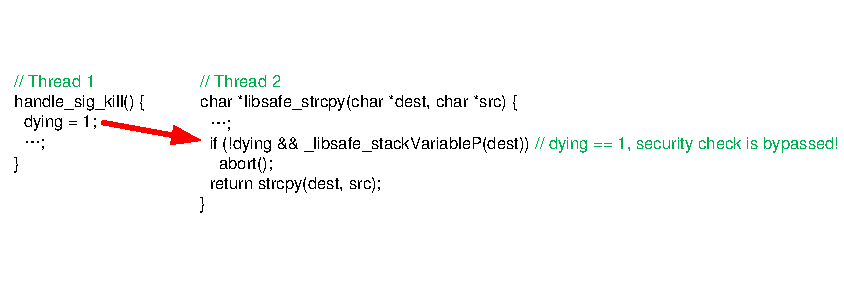
\includegraphics[width=0.8\columnwidth]{figures/libsafe}
\vspace{-.05in}
\caption{{A concurrency attack in the Libsafe security library.}} 
\label{fig:libsafe}
\vspace{-.15in}
\end{figure}

Figure~\ref{fig:libsafe} shows the code of a concurrency attack in 
\libsafe, a popular stack overflow protection library. This library 
provides its own safe memory and string operations functions. For instance, the 
\texttt{libsafe\_strcpy()} function checks whether a stack variable is passed 
in as the function argument \texttt{dest} before it calls the actual 
\texttt{strcpy()}. If a program receives a kill signal, Libsafe's internal 
thread (thread 1) sets a global variable \texttt{dying}, then security checks 
are disabled in \texttt{libsafe\_strcpy()}. Unfortunately, \v{dying} was not 
protected by mutex locks. In our study, we triggered a data race on this 
variable, bypassed the security check, and overflowed thread 2's stack by 
passing malicious code to \texttt{dest}. Ironically, this \libsafe library is 
no longer ``safe" when facing concurrency attacks.

\begin{figure}[h]
\centering
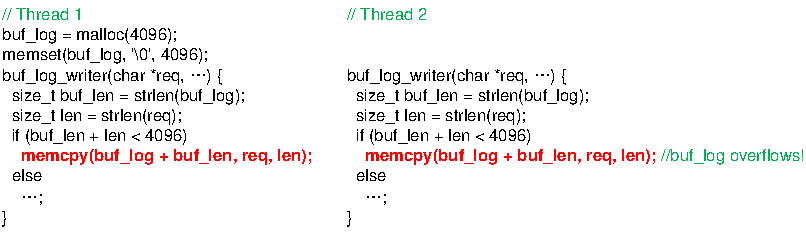
\includegraphics[width=0.8\columnwidth]{figures/apache}
\vspace{-.05in}
\caption{{A concurrency attack in the \apache web server.}} \label{fig:apache}
\vspace{-.15in}
\end{figure}

Figure~\ref{fig:apache} shows the code of a concurrency attack in 
the widely used \apache web server for maintaining users' HTTP pages. \apache 
spawns a number of threads, each serves a HTTP request. Each thread also records 
the request in a global log buffer in heap and flushes this buffer to a log 
file when the buffer is full. However, developers missed a mutex lock to 
protect this buffer, so the buffer can overflow and corrupt adjacent memory, 
including the log file's descriptor. In our study, we corrupted this descriptor 
and made \apache write a request record to mess up another user's HTTP page.



\vspace{-.15in}\subsubsection{Concurrency Attack Model} 
\label{sec:attack-phase}\vspace{-.075in}

A key question on modeling concurrency attack is: how does the corrupted memory 
in a concurrency bug propagate to vulnerable instructions in souce code? Since 
existing reliability tools (\S\ref{sec:others-work}) are already effective on 
detecting concurrency bugs, if our model can address this question, we can 
effectively identify which concurency bugs have the potential to lead to 
attacks, and we can safely ignore those don't.

% P3: pattern.
Although the two aforementioned examples appear to be diverse, we have 
identified three common elements in these concurrency attacks. First, it is 
necessary to have corrupted global memory (\eg, \texttt{dying} in \libsafe, and 
the \texttt{buf\_len} in \apache) caused by concurency bugs. Second, it is 
necessary to have a vulnerable instruction (\eg, \texttt{strcpy()} or 
\texttt{setuid()}) to perform an attack. Third, the corrupted values in global 
memory must cause abnormal behavior on the vulnerable instructions. For example, 
the abnormal behavior in \libsafe is we must leverage the corrupted memory to 
bypass the stack overflow check, an abnormal control-flow of the execution. For 
\apache, we must directly corrupt (\ie, overflow) the buffer log, an abnormal 
data-flow of the execution.

% In sum, three common elements compose a concurrency attack model: corrupted 
% memory, security-sensitive operation, and impact (indirect or direct) from the 
% memory to the operation.
% 
In addition to these two examples, the \nattacks concurrency attacks in recent 
study~\cite{con:hotpar12} and the \noldattacks ones our own preliminary study 
\S\ref{sec:examples}) also have the three common elements. For the first 
element, these attacks have four types of concurrency bugs, including data 
races, atomicity violations, deadlocks, and order violations. For the second 
element, we have collected three types of vulnerable instructions, including 
memory operations (\eg, \texttt{strcpy()}), pointer deferences (\eg, when the 
pointer is NULL), and systems calls (\eg, \texttt{setuid()}). For the third 
element, the key is to detect abnormal control-flow and data-flow of 
executions, and \S\ref{sec:detect} will proposse our systematic detection 
approach.

% PX: emphasis the contribution/potential value of this model.
% In a high level, this model treats a concurrency attack as a source-sink model, 
% where a source is a corrupted global memory caused by a concurrency bug, and a 
% sink is a security-sensitive operation. Then this model tracks the data flow 
% and control flow of the corrupted memory to the sensitive operations. Unlike a 
% traditional model which only consider inputs as the source, our model considers
% concurrency bugs as the the inputs. This model spurs several interesting 
% research questions. First, how do we track down the corrupted memory in the 
% middle of an execution? Second, given that concurrency bugs are not only just 
% one, how does our analysis handle multiple concurrency bugs (\eg, multiple 
% corrupted variables)? Third, given that not all security-sensitive operations 
% are indeed relevant to the source, how do we prune the irrelevant operations 
% soundly (\ie, without missing exploits)? In \S\ref{sec:detect}, we plan to 
% leverage this model to develop an effective detection approach, and our 
% preliminary work has shown promising results on addressing these research 
% questions.

% TBD: add a table on the list of concurrency bugs and the list of dangerous 
% operations.



% P5: how to handle unknow patterns? Just say patterns in our work may spur new 
% patterns. We will continue to find new patterns as well.
% P5: TBD.

% \subsubsection{Concurrency Attacks with Three Common Patterns}
% \label{sec:model-pattern}

% Goal 1: modeling.

\vspace{-.15in}\subsection{Objective 2: Detecting Concurrency Attacks in 
Testing Phase}\label{sec:detect}\vspace{-.075in}

We aim to build a concurrency attack detection tool for developers in the 
testing phase. This tool takes program source code as input, and it reports 
whether this program has potential concurrency attacks. Even for old releases 
of programs, this tool is still helpful, because attacks are consequences of 
bugs, even if the bugs were already fixed, if the attacks have occurred, fixing 
the bugs do not help. For example, we studied a few concurrency bugs in old 
Linux and BSD releases a few years ago, and their attacks are still helpful 
because if attackers have broken in and gain root privilege, simply fixing the 
bugs or upgrading kernels can not remove the malicious root user.

\vspace{-.15in}\subsubsection{Workflow of \xxx's Detection Scheme}
\label{sec:detect-arch}\vspace{-.075in}

An effective concurrency attack detection tool should meet a few goals. First, 
a concurrency attack report should contain preconditions on inputs of the 
programs so that developers can easily inspect. This goal is especially useful 
for developers to triggering attacks on rare inputs (\eg, mention the nested 
select inputs in MySQL).

Second, this tool should be precise in terms of having as few as false 
positives (reports but actually not a feasible attack) and false negatives 
(missing a real attack). A precise tool will encourage adoptions by the 
software developers. To this end, this tool must precisely capture both the 
data flow and control flow between the corrupted global memory and any 
potential security-sensitive operations in program source code. 

Our key weapon to achieve the first goal is \emph{symbolic execution}, an 
advanced program analysis technique that can systematically explore program 
paths to find bugs. Unlike normal execution which runs on a concrete 
inputs, this technique marks inputs (\eg, command lines and bytes received from 
network) as symbolic, and if a branch statement depend on inputs, it forks the 
execution, goes down both paths, and tracks constraints on inputs. If this 
technique hit a bug, the constraints on inputs reflect on input conditions 
which can trigger this bug. This technique has shown to find subtle bugs in 
real-world programs.

Our key weapon to achieve the first goal is path slicing, an advanced program 
analysis technique that. Given a trace of executed instructions and one 
instruction in this trace, this technique goes backward compute a subset of 
instructions that are necessary to determine the reachability and values of 
operands of this instruction.

\begin{figure}[ht]
\centering
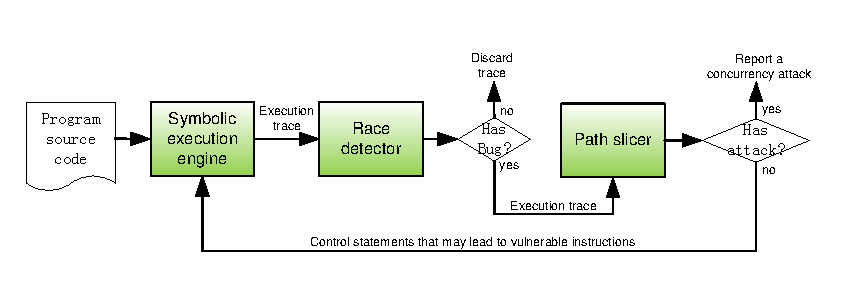
\includegraphics[width=0.5\columnwidth]{figures/detection}
\vspace{-.05in}
\caption{{Workflow of the concurrency attack detection scheme.}} 
\label{fig:detection}
\vspace{-.05in}
\end{figure}

With both the symbolic execution and path slicing tools, we plan to build a 
concurrency attack detection tool. The workflow of the tool is shown in 
Figure~\ref{fig:detection}. This tool takes program source code as input and 
uses the LLVM compiler framework to compile it to LLVM IR instructions. The 
symbolic execution engine marks a program input and bytes received from network 
as symbolic and explore program paths. For each program path, we run a race 
detector on the execution trace, and if a concurrency bug is detected, we feed 
this trace to path slicer to see whether it may lead to a dangerous operation 
or have any branch statements that can lead to dangerous operation. If the 
trace does not contain any bug, we discard this trace.

The path slicer takes a trace which contains a concurrency bug. The slicer 
first sees whether this trace has a dangerous operation, if so, it reports a 
potential concurrency bug with input preconditions. If not, the path slicer 
starts from the last execution of the trace, goes backward, and see whether a 
branch statement in this trace may lead to a dangerous operation. If so, it 
marks this branch as relevant. After processing this trace, the path slicer 
feed these branches to the symbolic execution engine, so that the engine can 
focus on exploring paths on these branches to try to exercise dangerous 
operations.

% P1: why need a detection scheme. First, capture as many as exploits in 
% testing phase. And call for re-install if there is any potential exploit. 
Even for 
% old concurrency bugs, it is still necessary because exploits may have already 
% occured and attackers may have already broken in.

% P2: two research questions. Given a concurrency bug, will it lead to an 
% exploit?

% P3: if this bug may lead to an exploit, what inputs may lead to such exploits?

% P4: how to incorporate the patterns in previous section?

% P5: go over the workflow, which is a straight line of boxes. May add some 
% back edges to make it an iterative approach?
 
% \subsubsection{Implementing \xxx's Detection Scheme}\label{sec:detect-impl}
% TBD

\vspace{-.15in}\subsubsection{Preliminary Results}
\label{sec:detect-result}\vspace{-.075in}

% P1: we have implemented part of the dangerous operation. pointer NULL 
% derefence. Report the results. FP:FN. 
My collaborators and I have built one basic building block of this detection 
tool, the path slicer called Woodpecker~\cite{woodpecker:asplos13} in ASPLOS 
2013. Woodpecker detects 113 programming rule violations in 136 popular systems 
programs, including 10 serious data loss errors with 2 most serious ones 
already confirmed by the corresponding developers. My collaborators and I have 
built a data race detector in our Tern~\cite{cui:tern:osdi10} in OSDI 2010 and 
Peregrine~\cite{peregrine:sosp11} paper in SOSP 2011. We believe these 
preliminary results show the potential and practical impact of our proposed 
detection tool.

% P2: mention our initial work in OSDI '10 and SOSP '11 on precise data race 
% detection.


% P2: we foresee a few open challenges on the continuation of developing this 
% tool. First, how to make path slicing handle % non-function calls. Second, 
how 
% to prioritize different operations ()? % Third, how to select malicious 
% inputs and thread schedules that are more likely to triger concurrency bugs?
We foresee a few open challenges on the continuation of developing this tool. 
First, how to make path slicing handle non-function calls (\eg, NULL pointer 
dereference). Second, how to prioritize different operations (\eg, some 
\v{strcpy} functions do not involve with inputs and should be secure)? Third, 
how to direct our symbolic execution engine to select malicious inputs and 
thread schedules that are more likely to trigger concurrency bugs? I believe 
these challenges will continue to lead to significant work in good conferences.

\vspace{-.15in}\subsection{Objective 3: Defensing Concurrency Attacks in 
Deployment Phase} 
\label{sec:defense}\vspace{-.075in}

% P1: motivation, why runtime detection is important. We want to mostly avoid 
% exploits by preventing attackers from manipulating the schedules.
Although \S\ref{sec:detect} has proposed an detection scheme for developers to 
find concurrency attacks in the testing phase, this scheme can not catch 100\% 
attacks because it is designed to find attacks on the concurrency bugs it meets 
at runtime. Thus, to practically prevent concurrency attacks taking over 
multi-threaded programs in the deployment phase, an efficient, transparent 
runtime infrastructure is needed to defense concurrency attacks.

% P2: reason 2: when races occur even if Parrot is enforced, we want to have 
% fault-tolerance.
To build a defense infrastructure, I propose to leverage state machine 
replication (or \smr), a powerful fault-tolerance concept in today's 
distributed system and clouds. \smr models a program as a deterministic
state machine, where the states are important program data and the transitions 
are deterministic executions of program code under input requests. SMR runs 
replicas of the program and invokes a distributed consensus protocol 
(typically \paxos) to ensure the same sequence of input requests for replicas, 
as long as a quorum (typically a majority) of the replicas agrees on the input 
request sequence. Under the deterministic execution assumption, this quorum of 
replicas must reach the same exact state despite various exceptions such as 
program failures or network partitions. SMR is proven safe in theory and 
provides high availability in practice.

The fault-tolerant benefit of \smr makes it particularly attractive
on implementing a principled replication system for tolerating concurrency 
attacks. Unfortunately, doing so is quite challenging, and I foresee four 
challenges.

% P3: reason 3: we want survive. checkpoint and re-execute, and diversify the 
% schedules before re-execute. Sell it like a self-healing runtime system.
First, today's multithreaded programs are almost universally
multithreaded, thus even concurrency attacks do not manifest, the programs 
running across replicas can still easily run into different thread schedules 
and divergent execution states. Second, to leverage existing SMR systems such 
as ZooKeeper, developers often have to shoehorn their programs into the 
narrowly defined state machine interfaces provided by these SMR systems. Third, 
such a runtime infrastructure should run almost as fast as the native 
executions in the deployment phase. Fourth, if replicas run into buggy 
schedules that trigger concurrency attacks, our infrastructure should be able 
to recover from the attacks.

\vspace{-.15in}\subsubsection{Architecture of \xxx's Runtime Defense 
Infrastructure} 
\label{sec:defense-arch}\vspace{-.075in}

\begin{figure}[ht]
\centering
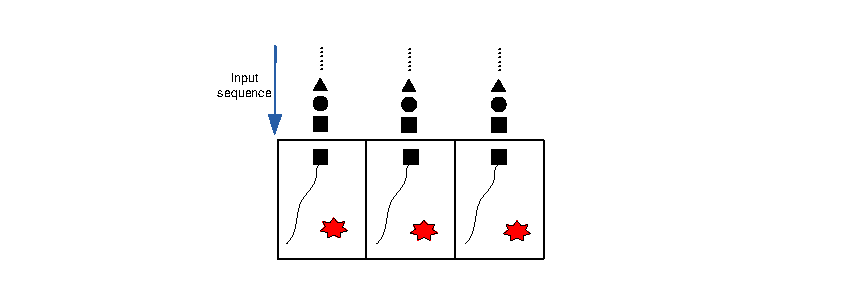
\includegraphics[width=0.3\columnwidth]{figures/defense}
\vspace{-.05in}
\caption{{A runtime infrastructure to defense concurrency attacks.}} 
\label{fig:defense}
\vspace{-.05in}
\end{figure}

To address these challenges, I propose a \smr-based replication 
system. With this infrastructure, a developer focuses on implementing her 
program's intended functionality, not how to defense concurrency attacks. When 
she is ready to replicate her program for strengthened security, she simply
runs this infrastructure with her program on multiple replicas. Within
each replica, this infrastructure interposes on the socket and the thread
synchronization interfaces to keep replicas in sync. Specifically, to address 
the first challenge, it considers each incoming socket call (e.g., accept() a 
client's connection or recv() a client's data) an input request, and runs a 
\paxos consensus protocol to ensure that a quorum of the replicas sees the same 
exact sequence of the incoming socket calls.

To address the second challenge, this infrastructure schedules synchronizations 
using deterministic multithreading (DMT). This technique
typically maintains a global, monotonically increasing logical clock that 
advances deterministically on each thread's synchronization. By serializing 
thread synchronizations, DMT practically makes an entire multithreaded 
execution deterministic. The overhead
of DMT is typically moderate because most code is not synchronization and can 
still run in parallel.

\begin{figure}[ht]
\centering
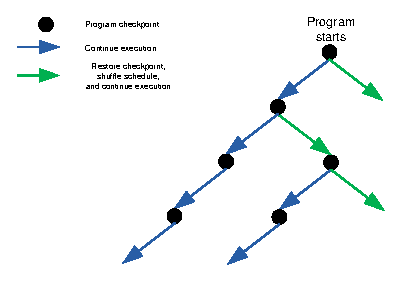
\includegraphics[width=0.3\columnwidth]{figures/healing}
\vspace{-.05in}
\caption{{The self-healing idea for recovering from concurrency attacks.}} 
\label{fig:healing}
\vspace{-.05in}
\end{figure}

% Mention the self healing idea.
To address the fourth challenge, we propose a self-healing idea 
(Figure~\ref{fig:healing}), which leverage existing transparent program 
checkpoint and restore techniques. On program starts, one backup replica first 
checkpoints the program, and then the program runs as is. Once minor replicas 
hit concurrency attacks, the other replicas can still agree on new inputs and 
process requests. If all replicas fail due to hitting the same vulnerable 
schedule, we simply extracts a previous checkpoint, shuffle the schedules, and 
then let the program continues to execute. To this end, this idea checkpoint 
and recovery must work with general programs with its file system. To this end, 
it leverages CRIU to checkpoint and restore process states, and LXC for file 
system states.

As a typical security setting, we need to define which components of 
this Infrastructure must be trusted. In this project, we require the 
infrastructure and the checkpoints are trusted (\ie, even if the program 
compromises, its program checkpoints and the infrastructure are not effected). 
We consider this requirement as reasonable, because once this infrastructure is 
built, we can leverage existing verification techniques to focus on verifying 
this infrastructure, and on top of it, we no longer need to verify those 
programs.




% P4: challenges on doing so. Including the initial work.

\vspace{-.15in}\subsubsection{Preliminary Results} 
\label{sec:defense-result}\vspace{-.075in}

% P1: we have built a replication system. Perf and checkpoint results.
My collaborators and I have built a prototype system~\cite{crane:sosp15} to 
address the first two challenges. \crane has shown to be able to transparently 
and efficiently support four general multithreaded programs without modifying 
them. We have also shown that this infrastructure is robust on primary replica 
or backup failures. For the third challenge, we plan to study more 
programs and see whether we can leverage performance hints to optimize 
performance. For the fourth challenge, our prototype system \crane has 
implemented a basic checkpoint/restore feature.

\vspace{-.15in}\subsection{Research Plan} \label{sec:plan}\vspace{-.075in}

This \xxx project will require two PhD students S1 and S2 for a period of 
three years. In the first year, S1 will develop and refine the concurrency 
attack model (Objective 1), and S2 will leverage the model to design the 
detailed workflow of the detection approach (part of Objective 2) by working 
closely with S1. In the second year, S1 will do an emperical study on how well 
the model represents real-world concurrency attacks, and S2 will implement 
the detection approach as a software tool (part of Objective 2). In the third 
year, S1 will build the runtime defense infrastructure (Objective 3), and S2 
will apply our model, detection tool, and defense infrastructure to benefit 
other research areas (\eg, byzantine fault tolerance). Overall, both the two 
students will involve theoretical methods, implement real software systems, and 
perform real-world study. The PI will supervise the students by providing 
advice 
concerning both theoretical and systems implementation levels.




% \pagebreak

\newpage
\AtBeginShipout{%
\AtBeginShipoutDiscard
}

\bibliographystyle{abbrvnat}
\bibliography{bib/biblio}

\end{document}


